%% The following is a directive for TeXShop to indicate the main file
%%!TEX root = diss.tex

\chapter{Luminescence from Organic Molecules}
\label{ch:opv}

Prior to the work done in this thesis, \ac{STML} from a single organic molecule has not yet been detected on our system. To optimize and ensure the viability of the experimental setup, \ac{STML} was performed on prototypical organic semiconducting molecules \ac{PTCDA} \citep{Rzeznicka2011, Kimura2019} and \ac{ZnPc} \citep{Zhang2016, Doppagne2017, Zhang2017, Imada2016, Doppagne2018, Miwa2019}, both of which have had successful reports of \ac{STML} experiments. Fluorination of phthalocyanine molecules have previously been demonstrated as a method to tune the electronic and optical energies of the molecule in bulk \citep{schwarze2016band, warren2019controlling}. Further experiments were carried out on \ch{F8ZnPc} to explore the effects of fluorination on the structural, electronic and optical properties of ZnPc.

During \ac{STML} experiments, the tip was parked on top of the molecule with a certain bias, and setpoint current. The shutter to the spectrometer was then opened for a certain exposure time $t_x$. The parameters for each \ac{STML} experiment will be listed as $V_b/I_t/t_x$.


\section{Plasmon emission from substrates}

Plasmon emission from the bare metallic surface can vary in energy and intensity depending on the geometry of the tip. Aside from attaining a sharp metallic tip for \ac{STM} and \ac{STS}, the tip needs to be poked and pulsed until it produce a strong plasmonic response in the energy region of interest. Representative spectra of the plasmon on Ag(111) and Au(111) with Ag tip is presented in \autoref{fig:opv:metal-plasmon}. The same Ag tip was used to acquire both spectra, allowing for comparison. Due to the shift in tip-sample junction on Au(111), a result of the thinner substrate, the plasmon emission intenisty was lower by about an order of magnitude when compared to the Ag(111) substrate. The red-shift in photon energy was caused by the inherent dielectric response of the gold substrate \citep{olmon2012optical, yang2015optical}. 

% The shift in photon energy was because of the dielectric function of the two materials: gold with a minimal imaginary dielectric function at \SI{1.8}{eV} or \SI{680}{nm} \citep{olmon2012optical}, and silver at \SI{3.2}{eV} or \SI{390}{nm} \cite{yang2015optical}.

\begin{figure} [h]
    \centering
    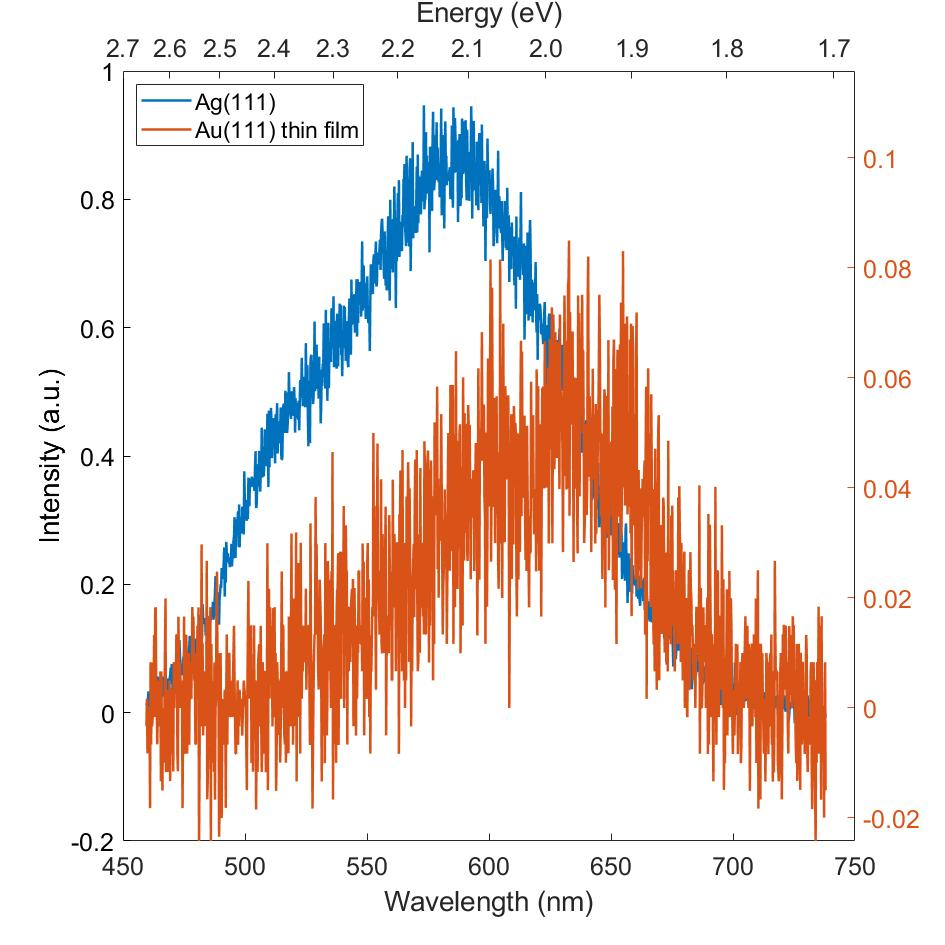
\includegraphics[width=4in]{pictures/Ag_Au_plasmon_3V_200pA_10s.jpg}
    \caption{\FIXME{Ag and Au plasmons, spectra taken with the same tip.}}
    % 573.3192 Ag, 632.7994 Au
    \label{fig:opv:metal-plasmon}
\end{figure}



When \ac{STML} experiments were carried out on molecular species, they were decoupled by a bilayer (2\ac{ML}) NaCl, which could modify the plasmon emission. Using the same Ag tip, modification of the plasmon emission on Ag(111) by layers of NaCl can be seen in \autoref{fig:opv:nacl-plasmon}. Overall, there was an enhancement in the detected photons when compared to the bare metal substrate, likely due to the smaller tip-sample distance.


\begin{figure} [h]
    \centering
    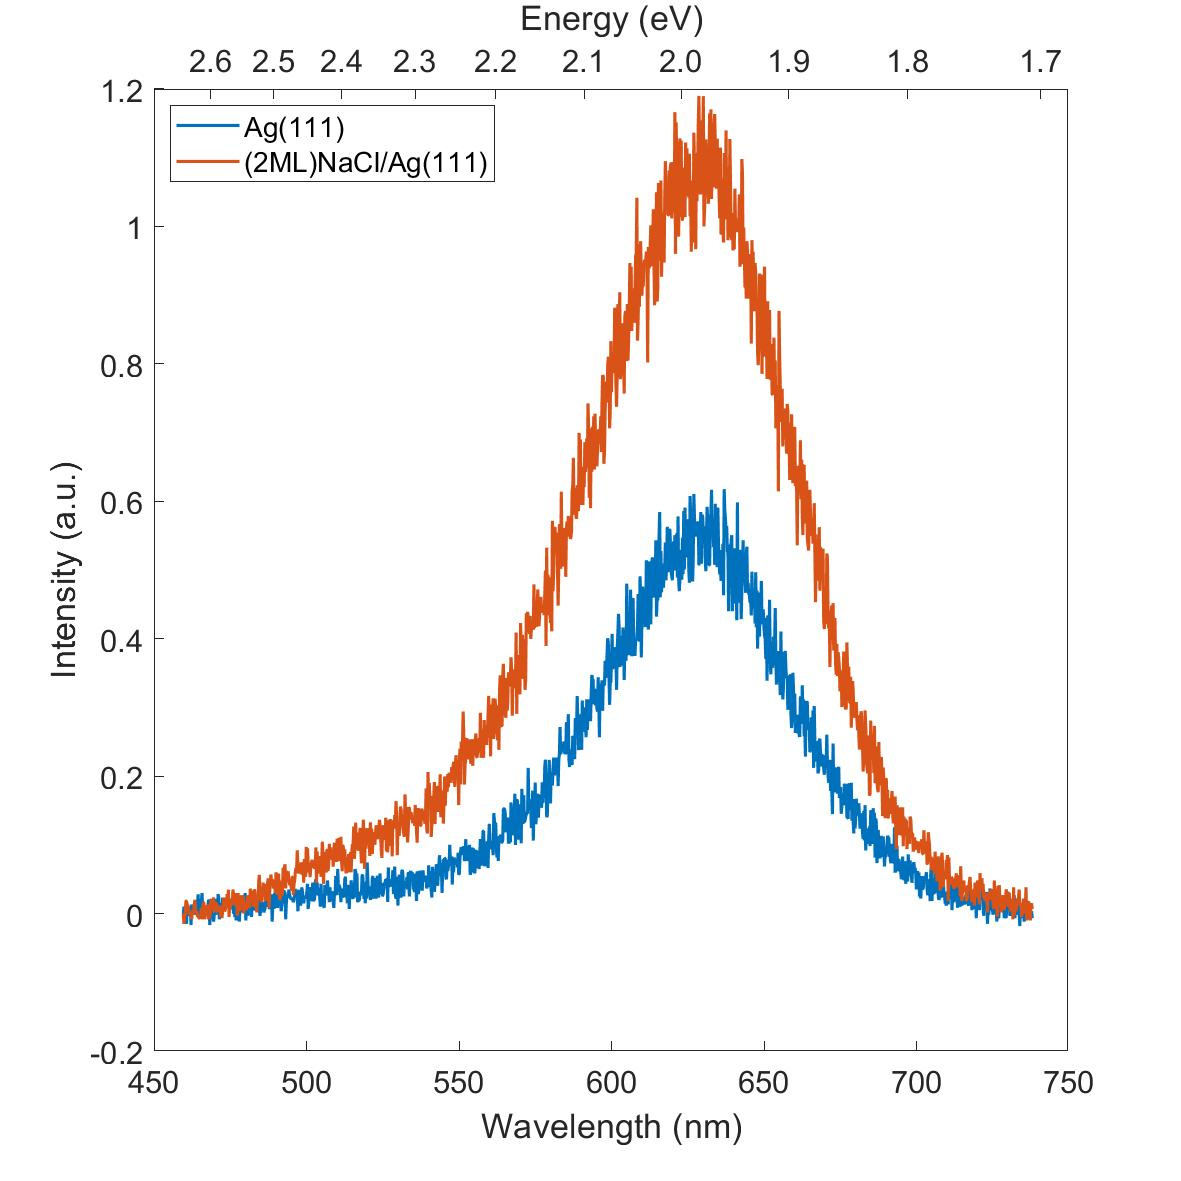
\includegraphics[width=4in]{pictures/NaCl_enhancement_Ag111_275V_250pA_10s.jpg}
    \caption{\FIXME{Ag and Au plasmons, modified by nacl (2ML and 3ML?)}}
    % 636.9401 Ag, 628.6561 NaCl/Ag
    \label{fig:opv:nacl-plasmon}
\end{figure}

Thicker layers of NaCl further dissociate the molecule from the metallic substrate, allowing for a more accurate study of the intrinsic properties of the molecule \citep{repp2005molecules}. Thicker layers of NaCl have also demonstrated enhanced molecular luminescence; the effect of a smaller tip-sample junction and more effective dissociation of the molecule from the metal \citep{Zhang2017,Kroger2018}. However, a closer tip results in stronger interactions between the tip and the molecule, affecting the stability of the molecule on the NaCl. Bilayer NaCl gave the most consistent and stable configurations for \ac{STML}.



\section{Study of {ZnPc}}

\ac{ZnPc} is a relatively planar organic semiconducting molecule that can be thermally deposited, making it optimal for \ac{SPM} study. To maximize \ac{STML} signal, ZnPc was deposited on (2ML)NaCl/Ag(111) and probed with the Ag tip. With parameters $\SI{3.0}{V}/\SI{300}{pA}/\SI{300}{s}$, we were able to detect emission from ZnPc at \SI{630}{nm} or \SI{1.96}{eV} (\autoref{fig:opv:znpc-stml}).

% Because of previous reports of \ac{STML} on ZnPc, this molecule was used to test the \ac{STML} capabilities of our system. 

% The structure of the ZnPc is shown in \autoref{fig:opv:znpc-stm}. The substrate was (2ML)NaCl/Au(111) thin film, and the tip used was the Pt/Ir tip dipped in gold. At biases higher than \SI{1}{V}, the ZnPc molecule rotates to give a 16-lobed structure. The non-rotating molecule has an 8-lobed structure, which could be seen if the molecules were ``anchored" by some defect or step edge, or was dimerized to another molecule.  

% \begin{figure} [h]
%     \centering
%     %\includegraphics[width=3in]{file}
%     \caption{\FIXME{Show stm of ZnPc (-1V, 1.0, 2.0), also with dimerize }}
%     \label{fig:opv:znpc-stm}
% \end{figure}

% The electronic structure was then probed using \ac{STS}. The \ac{LDOS} along with the molecular orbitals at the resonances are shown in \autoref{fig:opv:znpc-sts}.

% \begin{figure} [h]
%     \centering
%     %\includegraphics[width=3in]{file}
%     \caption{\FIXME{Show sts of ZnPc on Au(111)}}
%     \label{fig:opv:znpc-sts}
% \end{figure}

% Previous reports of ZnPc on this substrate show that the electronic states of the molecule do not change much in structure, and only experience a rigid shift of $\approx \SI{-1}{eV}$ in energy when compared to (2ML)NaCl/Au(111), due to the lower work function of (2ML)NaCl/Ag(111) \citep{Doppagne2017,Doppagne2018}. With an optimized Ag tip, photoluminescence was detected on the molecule, with an emission peak at \SI{630}{nm} or \SI{1.96}{eV} (\autoref{fig:opv:znpc-stml}).



\begin{figure} [h]
    \centering
    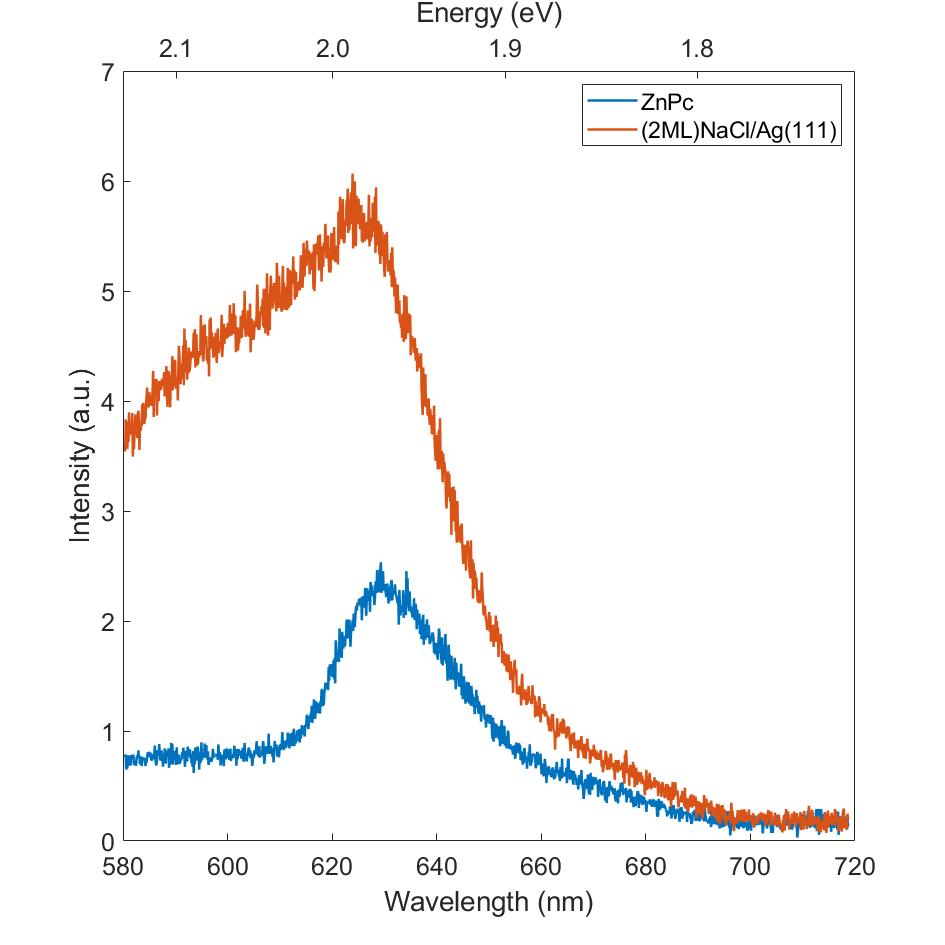
\includegraphics[width=3.5in]{pictures/znpc_3V_300pA_300s.jpg}
    \caption{\FIXME{show inset with the molecule on surface, and position of tip on molecule}}
    \label{fig:opv:znpc-stml}
\end{figure}

There are notable differences between our results and the results of previous reports of \ac{STML} on ZnPc \citep{Zhang2016, Doppagne2017, Zhang2017, Doppagne2018}. Previously reported photon peak energies are at \SI{652}{nm} or \SI{1.9}{eV}, while the peak energy in \autoref{fig:opv:znpc-stml} is higher in energy. Additionally, the peak in emission seen in \autoref{fig:opv:znpc-stml} is about four times broader, with \ac{FWHM} of about \SI{60}{meV}, while previously reported emissions have \ac{FWHM} of about \SI{15}{meV}.

The shift in energy and broadening of the molecular photoluminescence may be a result of the IR filters in place during our experiments. All \ac{STML} data was taken with the KG5 infrared filters in place, which have a transmittance cutoff in the range of the emission seen in \autoref{fig:opv:znpc-stml}. At around \SI{650}{nm}, the transmittance drops significantly to 50\% (\autoref{fig:expsetup:windows}), resulting in blue-shift and broadening of our signal. 

Additionally, in contrast to previously reported results taken at \SI{-2.5}{V}, we detected photoluminescence at a tip-sample bias of \SI{3}{V}. ZnPc has two equivalently stable adsorption angles on NaCl \citep{Miwa2016}, and rapid shuttling of between these geometries have been observed. At high positive biases, the ZnPc was noticeably more unstable, rotating more frequently seen as sub-\AA ngstr\"om jumps in the tip height. This instability and change in adsorption can change the geometry and vibrational modes of the ZnPc, suppressing the sharp 0-0 transition while favouring higher order vibrational excitations. 

Another factor that may explain the discrepancies observed is the presence of an alternative mechanism of molecular luminescence. Studies in the literature on \ac{STML} on ZnPc have described the emission to be the recombination of excitons formed by charge injection. However, at positive biases, charge injection exciton formation would require the Fermi level of the metal substrate to fall below the energy of the \ac{HOMO} of ZnPc in order to inject a hole into the system. Such a large shift is unlikely at a modest bias of \SI{3}{V}, and so the luminescence seen in \autoref{fig:opv:znpc-stml} may be a result of plasmon-mediated exciton recombination or some other molecular luminescence mechanism.








\section{Study of PTCDA}

The next system studied was the \ac{PTCDA} molecule on (2ML)NaCl/Au(111). As discussed before, the Au(111) thin film sample is slightly out of focus of the lens, resulting in weaker signals. However, \ac{PTCDA} is highly electronegative, and the (2ML)NaCl/Ag(111) substrate has a low work function, resulting in a charged PTCDA \citep{cochrane2017single,cochrane2018molecularly}. By using Au(111), which has a higher work function, as the metallic substrate, the PTCDA molecule was not charged on the surface, giving a simpler system to probe. Additionally, previous preliminary work in our group has demonstrated luminescence quenching on the PTCDA/(2ML)NaCl/Ag(111) system \citep{roussy2016coupling}, although a recent publication has shown luminescence at higher biases \citep{Kimura2019}.

Photoluminescence from a single PTCDA on (2ML)NaCl/Au(111) was detected, with an emission peak at \SI{670}{nm} or \SI{1.85}{eV}, at \SI{3}{V}/\SI{200}{pA}/\SI{300}{s} (\autoref{fig:opv:ptcda-stml}). The \ac{FWHM} of the peak is about \SI{90}{meV}, quite broad for single molecule emission. During the acquisition, the PTCDA shifted away, resulting in additional photon counts from the plasmonic emission. To compensate, the signal detected from the bare substrate was subtracted from the molecular luminescence.


\begin{figure} [h]
    \centering
        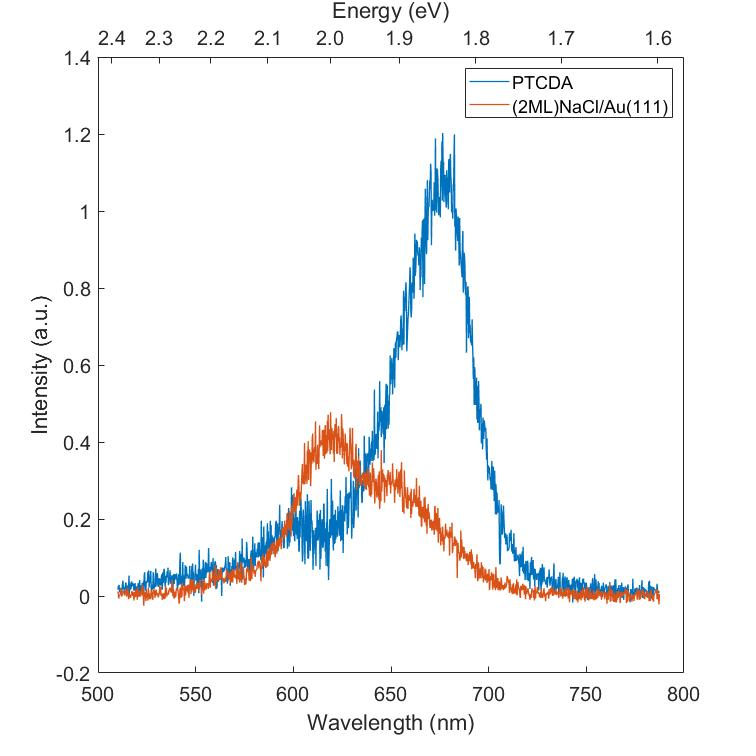
\includegraphics[width=3.5in]{pictures/ptcda_subtract_pl_3V_200pA_300s.jpg}
    \caption{\FIXME{show inset with the molecule on surface, and position of tip on molecule}}
    \label{fig:opv:ptcda-stml}
\end{figure}

There are significantly fewer \ac{STML} studies of PTCDA when compared to ZnPc. For comparison, we will refer to references \citep{Rzeznicka2011} and \citep{Kimura2019}. In the former, \textit{Rze\'znicka et al.} studied self-assembled bilayers of PTCDA on Au(111), with the first monolayer acting as the decoupling layer. The authors reported broad emission peaks at \SI{1.8}{eV} and \SI{2.35}{eV}, with FWHM of approximately \SI{100}{meV}, at a bias voltage of \SI{3}{V}. In the latter, \textit{Kimura et al.} studied single negatively charged PTCDA on (3ML)NaCl/Ag(111), detecting a sharp emission peak at \SI{2.45}{eV} with bias \SI{-3.4}{V}. 

The peak observed in \autoref{fig:opv:ptcda-stml} most closely resembles the lower energy \SI{1.8}{eV} emission seen by \textit{Rze\'znicka et al.}, who attributed the emission to the \ac{CT} exciton formed between the first and second monolayers of PTCDA. However, our system only consisted of a single isolated PTCDA molecule, with no neighbouring molecules to form a \ac{CT} complex. Additionally, the broadness seen by \textit{Rze\'znicka et al.} could be explained by the effects of adjacent molecules, but our isolated PTCDA system exhibits similar broadness in emissions, possibly due to the filtering effects of the IR windows. Regarding the higher energy photon emission, both publications attributed the higher energy peak to the $S_1 \rightarrow S_0$ 0-0 exciton recombination. However, we do not see this peak in our experiment, possibly due to the weak plasmonic enhancement in that region of the spectrum.

While the previous references are useful as comparisons, the studied PTCDA on (2ML)NaCl/Au(111) system was isolated and uncharged. The photoluminescence observed on this system may be the $S_1 \rightarrow S_0$ 0-0 exciton transition for a neutral PTCDA molecule. And, like the experimental parameters used for \ac{STML} on ZnPc, the photoluminescence was observed at a high positive bias of \SI{3}{V}. It is possible that tip induced conformational changes resulted in the suppression and enhancement of different vibrational transitions in the molecule. It is also possible that an alternative mechanism contributed to the emission seen in \autoref{fig:opv:ptcda-stml}, such as the plasmon-mediated exciton formation, or charge injection into LUMO+1 of PTCDA, forming an exciton between the LUMO+1 and LUMO which typically have a smaller optical gap \citep{Wu2008}. Due to the stability issues of PTCDA on NaCl at high biases, probing the LUMO+1 state by \ac{STS} was not performed.







% A recent work by \emph{Kimura et al.} was the first report of single molecule \ac{STML} on a negatively charged PTCDA, with a substrate of (3ML)NaCl/Ag(111). The authors corresponded the $S$ \FIXME{notation for the franck condon transitions} transition to an emission peak at \SI{2.45}{eV} with bias onset at $V_b=\SI{-2.2}{V}$ \citep{Kimura2019}. The energy of the emission peak seen in \autoref{fig:opv:ptcda-stml} does not correspond to the previously reported result. 

% Additionally, our detected emission is broadened, with a \ac{FWHM} of \SI{100}{meV}. The broadness and energy is similar to the \ac{CT} emission seen on the bilayer system, however, there were no neighbouring molecules in our system to broaden the signal or to form a \ac{CT} state. 

% An earlier study looked at \ac{STML} on a bilayer of \ac{PTCDA}, with the first monolayer acting as the decoupling layer. The authors found a broad \ac{CT} emission at \SI{1.75}{eV} for $V_b =\SI{2.5}{V}$, and an additional weaker $S_{10}$ transition at \SI{2.35}{eV} for $V_b = \SI{3.0}{V}$ \citep{Rzeznicka2011}. 

% A possible explanation for our spectra in \autoref{fig:opv:ptcda-stml} is the tunnelling






\section{Study of \ch{F8ZnPc}}

The energy of molecular orbitals can be tuned through halogenation, such as the introduction of fluorine into a molecular structure. Studies of fluorination on organic molecules have demonstrated the increase of electron affinity and ionization potential of molecules, effectively lowering the energy of HOMO and LUMO, and raising the Fermi level \citep{schwarze2016band,warren2019controlling}. Using \ac{STM}, the effects of fluorination could be understood at the single molecule level. Studying the fluorinated counterpart of ZnPc, \ch{F8ZnPc}, we can elucidate the effects of fluorination on the electrical and optical properties of the molecule.


\subsection{Luminescence on \ch{F8ZnPc}}

\ch{F8ZnPc} was thermally deposited onto (2ML)NaCl/Ag(111) and probed with a Ag tip. Using previously observed photoluminescence of ZnPc as an estimate, the tip plasmon was tuned to enhance primarily in the region of \SI{630}{nm}. With positive bias \SI{3}{V}/\SI{250}{pA}/\SI{60}{s}, a weak emission peak was detected at \SI{675}{nm} or \SI{1.83}{eV}, with FWHM of approximately \SI{50}{meV} (\autoref{fig:opv:f8znpc-stml_+}).

\begin{figure} [h]
    \centering
        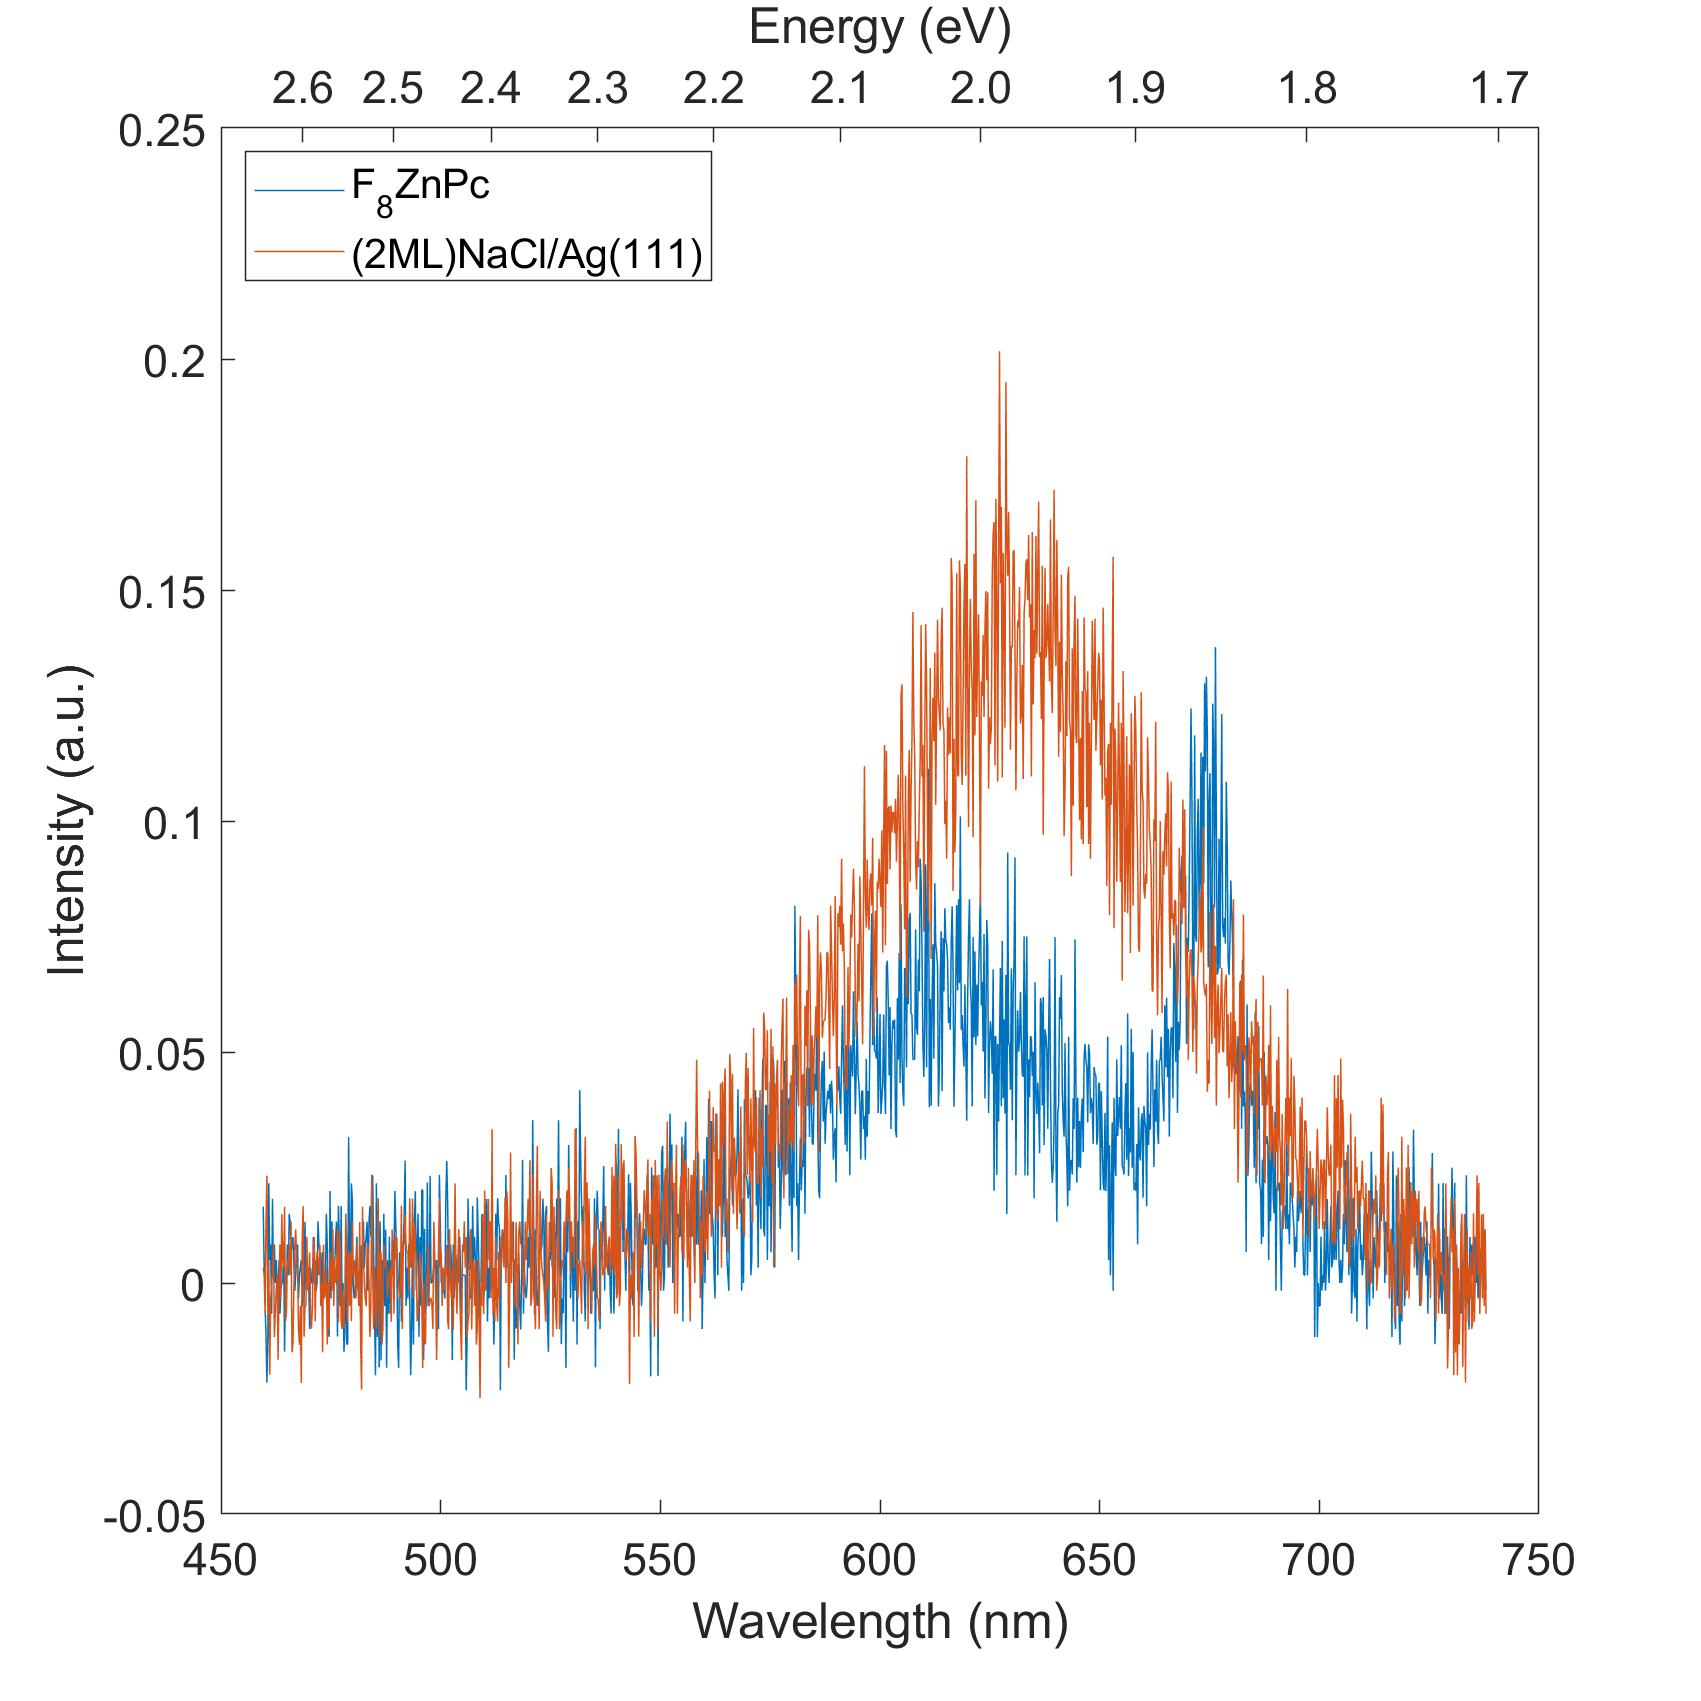
\includegraphics[width=3.5in]{pictures/f8znpc_3V_250pA_60s.jpg}
    \caption{\FIXME{show inset with the molecule on surface, and position of tip on molecule}}
    \label{fig:opv:f8znpc-stml_+}
\end{figure}

\ac{STML} was also conducted at negative bias for \ch{F8ZnPc}, and photoluminescence was detected at \SI{-2.5}{V}/\SI{200}{pA}/\SI{120}{s}. A strong and sharp emission peak was observed at \SI{640}{nm} or \SI{1.93}{eV}, along with well-resolved satellite peaks corresponding to vibrations transitions (\autoref{fig:opv:f8znpc-stml_-}). Higher resolution spectra was obtained with the \SI{600}{gr/mm} grating to better resolve the vibrational emission peaks. With the tip positioned above different parts of the molecule, changes in the vibrational satellite peaks were seen, but shifts in the energy of the 0-0 transition were minimal ($\sim \pm \SI{1}{nm}$). The strongest emission was observed with the tip positioned above the lobes of \ch{F8ZnPc}, and so all further experiments were performed at this location for maximal signal strength (\autoref{fig:opv:f8znpc-stml_600gr}).


\begin{figure} [h]
    \centering
    
     \begin{subfigure}{0.45\textwidth}
           %\includegraphics[width=4in]{pictures/2019_11_07_F8ZnPc_shifts_lobe-centre.svg}
        \caption{\FIXME{show inset with the molecule on surface, and position of tip on molecule}}
        \label{fig:opv:f8znpc-stml_-}
    \end{subfigure}
    
    \begin{subfigure}{0.45\textwidth}
        %\includegraphics[width=4in]{pictures/2019_11_07_F8ZnPc_shifts_lobe-centre.svg}
        \caption{Changes in vibration satellite peaks as the tip is positioned over different parts of the \ch{F8ZnPc}. Parameters used were \SI{-2.5}{V}/\SI{100}{pA}/\SI{300}{s}.}
        \label{fig:opv:f8znpc-stml_600gr}
    \end{subfigure}
    
    \caption{\FIXME{maybe don't include the bias dependence}}
    
\end{figure}

The differences between the positive and negative bias \ac{STML} results could be explained by the effects described in the previous section. \FIXME{can I postulate this?} A broad vibrational peak in the negative bias emission in \autoref{fig:opv:f8znpc-stml_-} coincides at the energy of around \SI{670}{nm}---the same energy as the positive bias emission peak in \autoref{fig:opv:f8znpc-stml_+}---giving evidence for preferred vibrational exciton transitions at positive biases.



\subsubsection*{Diversity in molecular types}

% introduce the different species problem

Surprisingly, the \ac{STM} scans at negative biases revealed a variety of topographically different molecules on the surface that were not previously seen at positive biases. To eliminate the possibility of fragmentation or degradation of molecules, a new sample of \ch{F8ZnPc} was loaded into the evaporator crucible, and the sample was prepared again. However, the same diversity was still present (\autoref{fig:opv:f8znpc-stm_diff}). Additionally, we were able to induce switching from one type to another with the tip, suggesting differences in the interaction between molecule and substrate as the cause for the distinct types. Possible reasons include the presence of defects or contaminants, and adsorption geometry of \ch{F8ZnPc} on the substrate.


\begin{figure} [h]
    \centering
        %\includegraphics[width=4in]{pictures/2019_11_07_F8ZnPc_shifts_lobe-centre.svg}
    \caption{\FIXME{image at positive and negative bias, demonstrating the diversity}}
    \label{fig:opv:f8znpc-stm_diff}
\end{figure}

Further \ac{STML} experiments at negative biases were conducted on the different types of \ch{F8ZnPc}, with $S_1 \rightarrow S_0$ 0-0 transition peaks varying from \SI{630}{nm} to \SI{643}{nm}. In order to correspond the emission peaks to the electronic states of the molecules, \ac{STML} along with \ac{STS} was performed on three of the observed types (\autoref{fig:opv:f8znpc-sts_stml}). With decreasing band gap, there is a corresponding decrease in the optical gap, observed as lower energy emission from exciton recombination. Further experimentation on this sample was not attempted due to the unstable nature of the Ag tip, making it unsuitable for high resolution \ac{STM} or \ac{STS}, and the wide variety of types of \ch{F8ZnPc} observed on the surface. 


\begin{figure} [h]
    \centering
        %\includegraphics[width=4in]{pictures/2019_11_07_F8ZnPc_shifts_lobe-centre.svg}
    \caption{\FIXME{grid and STML}}
    \label{fig:opv:f8znpc-sts_stml}
\end{figure}



\subsection{Adsorption geometry of \ch{F8ZnPc}}

To further investigate the adsorption geometry of \ch{F8ZnPc} on the substrate, the same sample was prepared after a full system vent and bakeout to ensure all contaminants in the chambers were purged. It was during this time that the new windows were installed (\autoref{fig:expsetup:windows}), but, due to time constraints, no additional \ac{STML} experiments were carried out. Instead, the Pt/Ir tip was used to probe the \ch{F8ZnPc} on (2ML)NaCl/Ag(111), giving consistent \ac{STM} and \ac{STS}.

Despite similar sample preparation conditions, there were clear differences between the sample used for \ac{STML} experiments, and the sample used to investigate the adsorption geometry of \ch{F8ZnPc}. The insulating NaCl layers were noticeably free of defects, and there were fewer types of \ch{F8ZnPc} after deposition, making classification more manageable. This suggests that some of the molecular variety may have been the result of underlying defects. 

\begin{figure} [h]
    \centering
        %\includegraphics[width=4in]{pictures/2019_11_07_F8ZnPc_shifts_lobe-centre.svg}
    \caption{\FIXME{STS with each type}}
    \label{fig:opv:f8znpc-sts_types}
\end{figure}

We identify four main stable types of \ch{F8ZnPc}, each with distinct topography and \ac{STS} resonances, as seen in \autoref{fig:opv:f8znpc-sts_types}. There were additional types but, due to rarity and molecular instability, they were not classified or examined in depth. The types were named in order of most to least abundant: T1, T2, T3, and T4. By scanning at high bias and current over types 2--4, the molecules were converted into T1, suggesting that T1 was the most stable configuration of \ch{F8ZnPc} on NaCl. 

Furthermore, the configuration of each type of \ch{F8ZnPc} relative to the underlying NaCl lattice was studied. For a small area of NaCl with a type of \ch{F8ZnPc}, the NaCl portion was scanned with high current and low bias to give an atomic resolution of the NaCl terrace. The scanning parameters were then restored when scanning over the molecule. The lattice was then drawn for the entire image, with the bright atoms corresponding to \ch{Cl-} ions \citep{heidorn2013influence}. The results for each type of \ch{F8ZnPc} are summarized in \autoref{fig:opv:f8znpc-atomic_types}.

\begin{figure} [h]
    \centering
        %\includegraphics[width=4in]{pictures/2019_11_07_F8ZnPc_shifts_lobe-centre.svg}
    \caption{\FIXME{sample image of atomic resolution}}
    \label{fig:opv:f8znpc-atomic_types}
\end{figure}


% why we didn't see it in ZnPc or PTCDA.
% talk about the images, and also the adsorption site



% talk about what we can relate back to ZnPc, T1 emission was observed. Furhter STML experimentation required on this new sample.



%%%%%
